% !TEX encoding = UTF-8 Unicode
%!TEX root = thesis.tex
% !TEX spellcheck = en-US
%%=========================================
\section{Experiment 2}
In this experiment, the aim is to find a good value for add link probability et al TODO

\subsection{Configuration}
\begin{minipage}{\linewidth}
\centering
\captionof{table}{Table Title TODO} \label{tab:title} 
\begin{tabular}{ C{3.5in} C{1.6in} }\toprule[1.5pt]
\bf Parameter & \bf Value \\
\midrule
  Number of generations & 50 \\
\midrule
  Fitness function & Local similarity \\
\midrule
  Target sound & Drum loop \\
\midrule
  Input sound & White noise \\
\midrule
  Effect & Distortion and resonant low-pass filter \\
\midrule
  Audio features & mfcc\_0, mfcc\_0\_\_derivative, mfcc\_1 \\
\midrule
  Number of runs & 400 per configuration \\
\bottomrule[1.25pt]
\end {tabular}\par
\bigskip
Should be a caption TODO
\end{minipage}

\subsection{Fitness function}
Same as in experiment 1

\subsection{Evaluation of configurations}
Figure \ref{fig:add_link_probability} TODO shows that 0.03 is probably the best value while 0.3 is significantly worse

\begin{figure}[h]
    \centering
    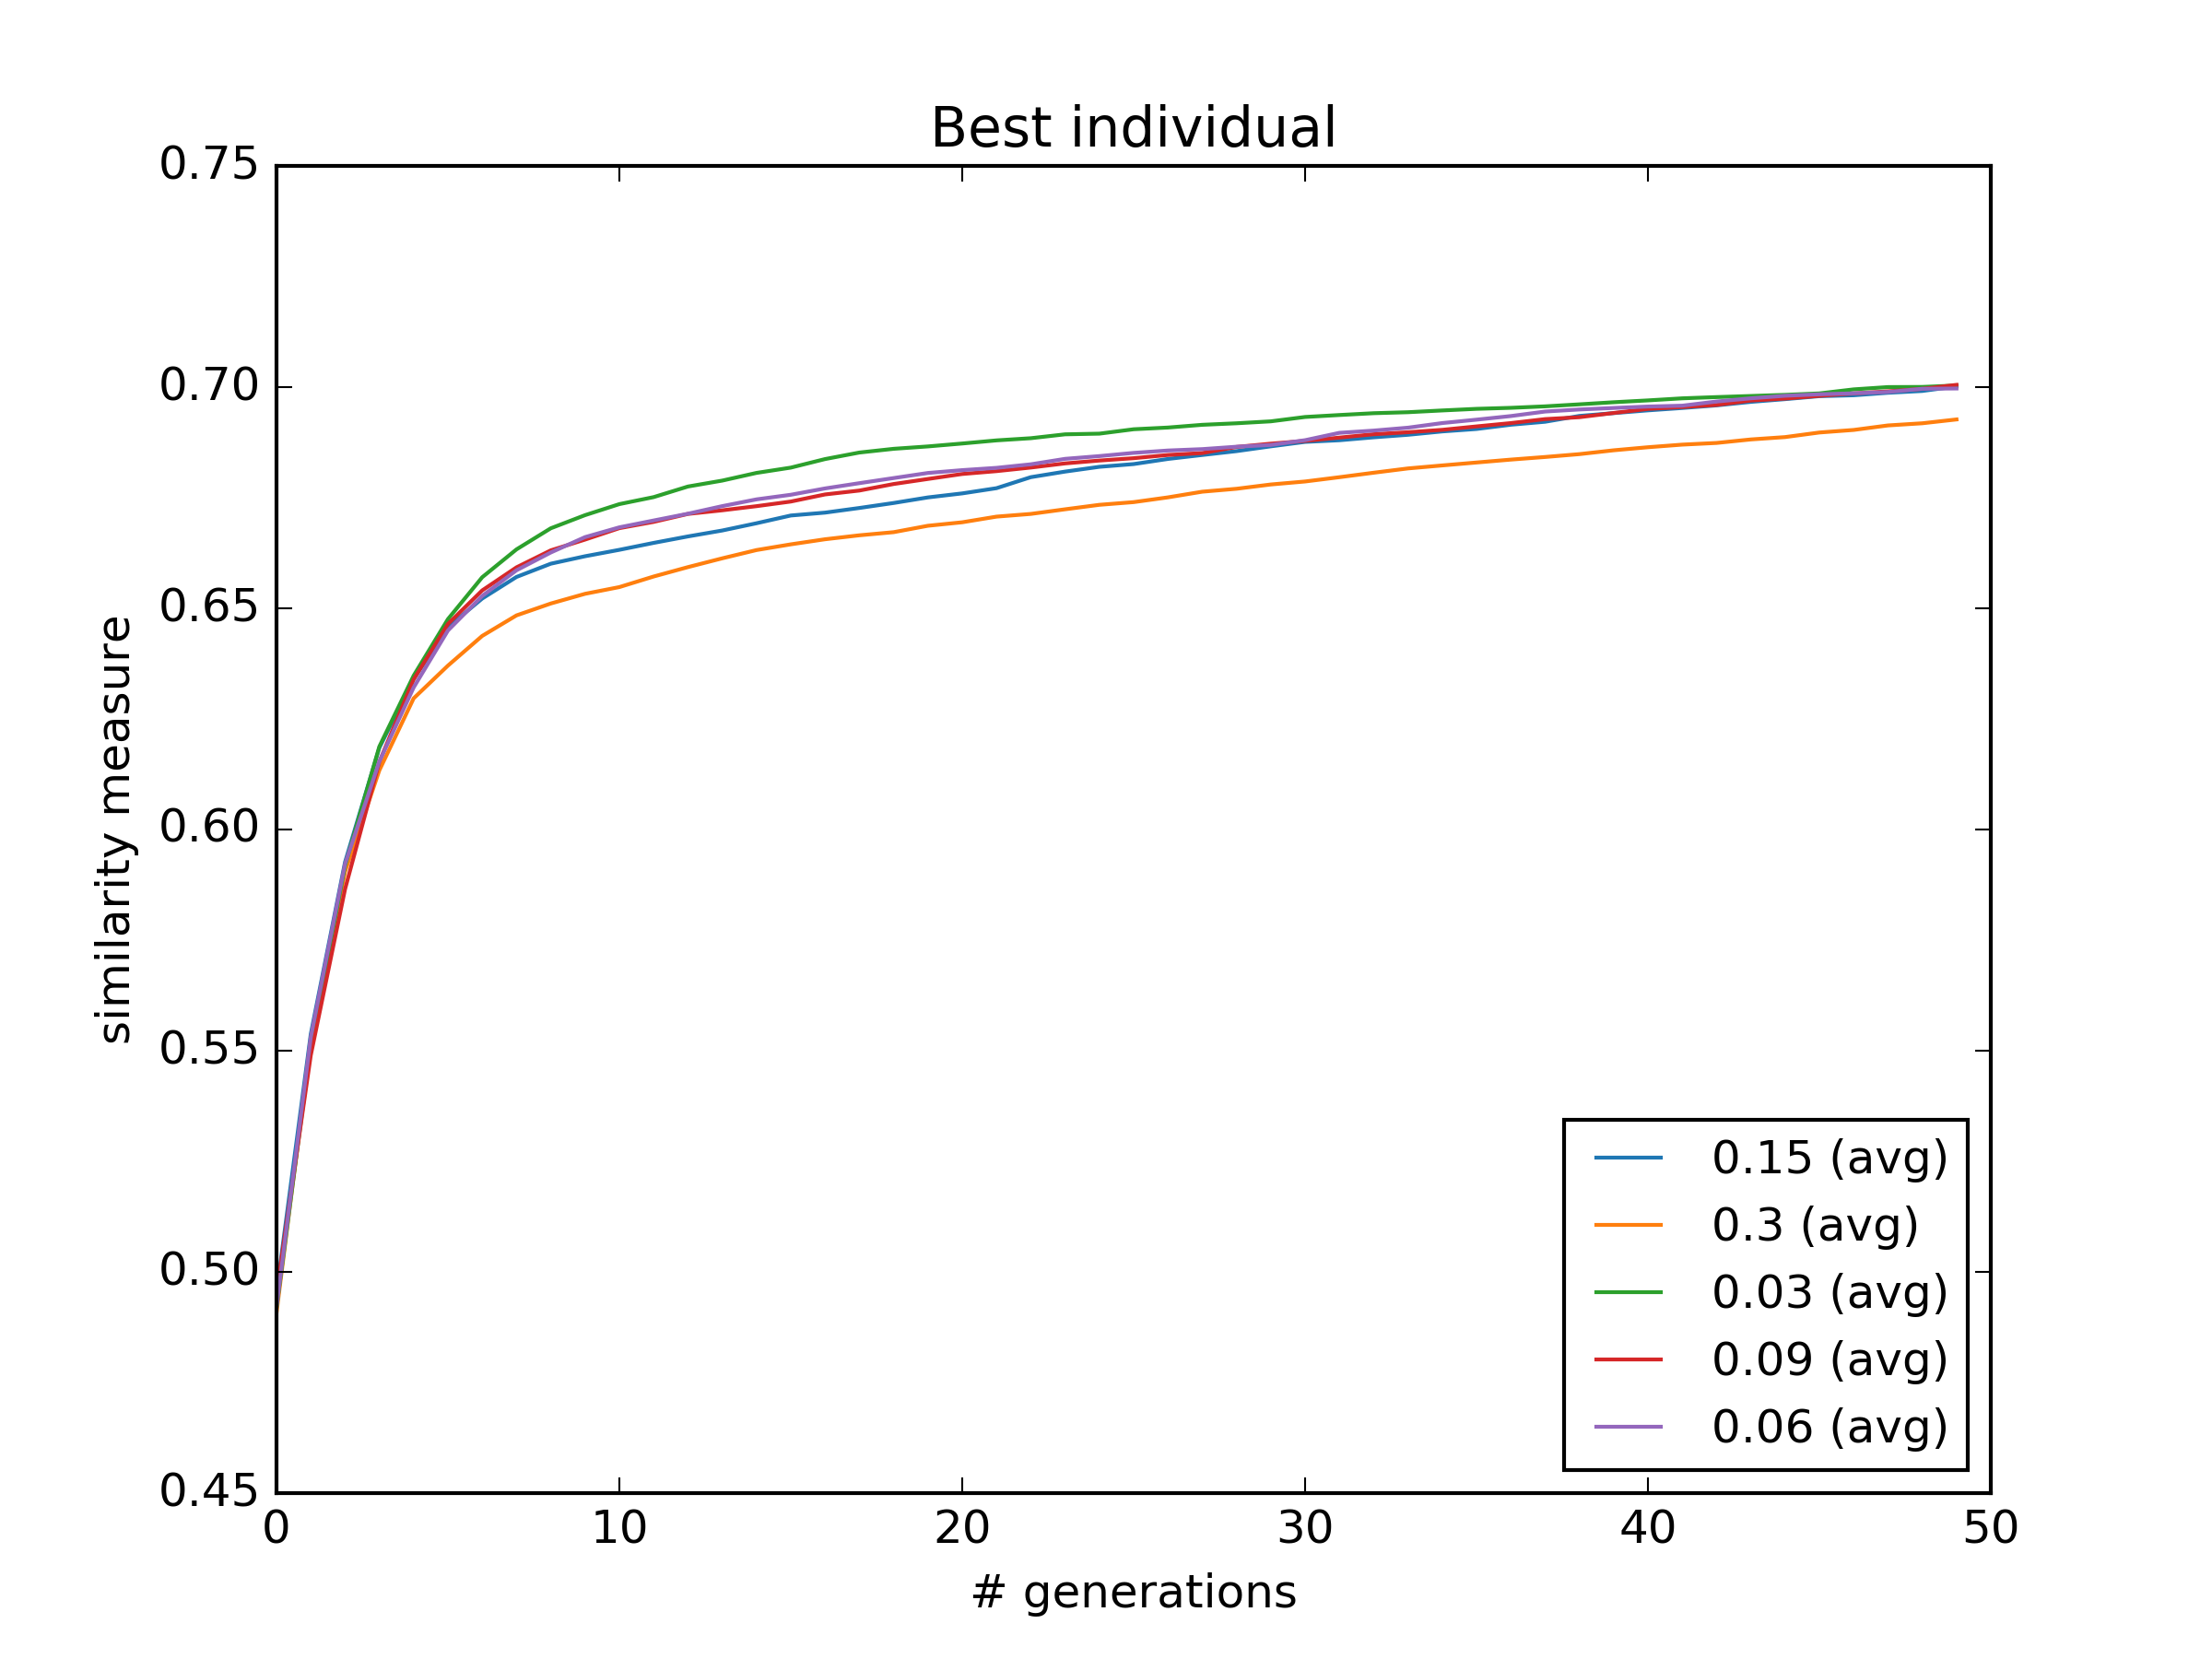
\includegraphics[width=0.99\textwidth]{add_link_probability}
    \caption{TODO caption}
    \label{fig:add_link_probability}
\end{figure}

TODO: Show typical end-result neural networks from all the configurations, to highlight that higher probability builds a larger, more complex network